\section{Closed Loop Drive Control}
\subsection{Introduction}
WTR currently has an "open loop control system" \cite{openloop} that controls how it turns and drives.
There are no sensors used to provide feedback, which could be used to control and adjust accordingly.
This is a major drawback, because the robot is already quite difficult to control; While it does not move very quickly, the motors have a lot of power behind them.
Should one of the wheels receive less power from the motor than the other, it will affect the trajectory of WTR, resulting in poor path-finding.

\subsection{System Description}
\label{subs::SysDes}
WTR consists of two powered wheels at the front and two wheels on pivot each at the rear.
The two powered wheels each have a separate electrical motor.
This set-up is quite sensitive to small variations between the two motors, though it does allow for a good range of movements.

\subsection{Current Setup}
An Arduino Mega 2560 (based on the ATmega2560 \cite{ardMega} is used to receive input from the laptop used as core control unit, and then translates that into instructions for the motors from the mobility scooter.
The commands sent are translated into a corresponding power output of the wheels via the integrated motor controller of the scooter.
Two commands can be sent, one for the speed of the motors and one for rotation.
Both commands fall within a range of 100 to -100.
Unfortunately, this set-up does not allow for independent control of both motors, but an appropriate model of the system could be used to approximate that level of control.

\subsection{Improvements}
Two sensors will be added to the axles of both wheels, which allow WTR to use the speed and rotation of the wheels as feedback.
These sensors will be controlled via a micro-controller, likely a Arduino Uno \cite{ardUno}, since those are already available and simple to use.
This set-up would allow for an integrated closed loop control system using negative feedback.
An overview can be found in figure~\ref{fig::cllp}.
\begin{figure}[H]
\centering
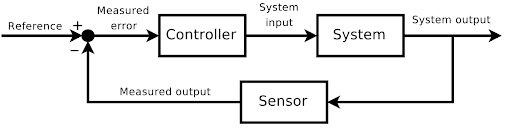
\includegraphics[width=12 cm]{controlmodel.png}
\caption{Example of the closed loop control system}
\label{fig::cllp}
\end{figure}
\newpage

\subsection{Model Of Control}
\subsubsection{Base}
As explained in 'System Description' \ref{subs::SysDes}, the motors can only be controlled through two output variables.
These two variables are \code{drive} output and \code{turn} output, both limited to values between 100 and -100.
Originally, these input were sent directly from the Arduino Mega, which applied the limits to the received values.
An overview can be found in table~\ref{tab::varoverview}
\begin{figure}[H]
\begin{tabular}{|l|l|c|c|l|l|}
\hline
\textbf{Nr.} & \textbf{Variable(s)} & \textbf{Left(+)} & \textbf{Right(-)} & \textbf{Min} & \textbf{Max} \\ \hline
1 & Input Turn 	& \multicolumn{2}{c|}{Turn\_ Input} 				& - 		& -		\\ \hline
2 & Input Drive 	& \multicolumn{2}{c|}{Drive\_ Input} 				& - 		& - 		\\ \hline
3 & Drive Output & \multicolumn{2}{c|}{Drive\_ Output = Drive\_ Input}	& -100 	& +100 	\\ \hline
4 & Turn Output 	& \multicolumn{2}{c|}{Turn\_ Output = Turn\_ Input}	& -100	& +100	\\ \hline
\end{tabular}
\caption{Overview of inputs and outputs of the original system}
\label{tab::varoverview}
\end{figure}

\subsubsection{Control Model}
To be able to create a controller which can control the speed of the wheels depending on input based on both the drive and input values, a direction definition has to be set up first.
The definition is:
\begin{itemize}
\item \code{Turning left will be a positive input value and a corresponding positive left wheel speed and a negative or lesser right wheel speed. Turning right will correspond with a negative input value and a positive right wheel speed and a negative or lesser left wheel speed}
\item \code{Moving forward corresponds with a positive input value and wheel speed, while moving backwards corresponds with a negative input value and negative wheel speed}
\end{itemize}
This is illustrated in figure \ref{fig::controldiagram}.
This system allows for a calculation of a separated reference speed per wheel, which is shown in table \ref{tab::closedoverview}, row 4.
The total reference speed can be calculated as shown in table \ref{tab::closedoverview}, row 5.
The offset per wheel (labelled as \code{Error}) can be calculated by subtracting the measured speed from the reference speed, as shown in table \ref{tab::closedoverview}, row 7.
As the speed of the wheels cannot be individually controlled, both errors have to be combined into the drive output and turn output variables.
Additionally, a controller $(C_m(S))$ has to be integrated.

\begin{figure}[H]
\centering
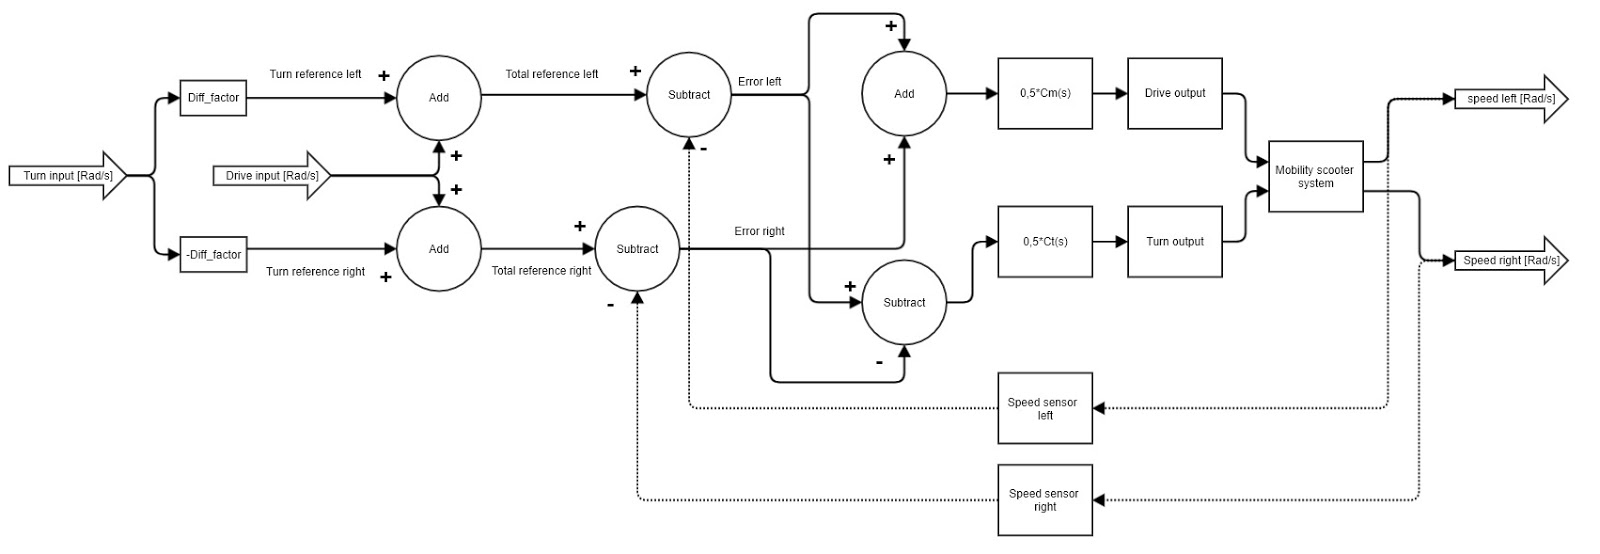
\includegraphics[width=15cm]{BlockDiagramCLCSR0.jpg}
\caption{Overview of the system integrated with closed loop control system}
\label{fig::controldiagram}
\end{figure}


\begin{figure}[H]
\begin{tabular}{|l|l|C{4cm}|C{4cm}|c|c|}
\hline
\textbf{Nr.} 		& \textbf{Variable(s)	}& \textbf{Left(+)}	&\textbf{Right(-)}							& \textbf{Min}	& \textbf{Max} 	\\ \hline
1		& Input Turn		& \multicolumn{2}{c|}{ Turn\_ Input}				& -		& -		\\ \hline
2		& Input Drive	& \multicolumn{2}{c|}{ Turn\_ Input}				& - 		& -		\\ \hline
3		& Reference Drive& \multicolumn{2}{c|}{ Drive\_ ref = Drive\_ Input}	& -		& - 		\\ \hline
4		& Reference Turn	&  $ Turn\_ Ref\_ L = Turn\_ Input * Diff\_ factor \footnote{difference in max speed of the wheel while turning compared to max speed while driving straight} $  & $ TUrn\_ Ref\_ R = -Turn\_ Input * Diff\_ Factor $ & - & - \\ \hline
5		& Total Reference Speed & $Tot\_ Ref = Drive\_ Ref + Turn\_ Ref\_ L$ & $Tot\_ Ref\_ R = Drive\_ Ref + Turn\_ Ref\_ R $ & -&- \\ \hline
6		& Measured\footnote{Sensors must be able to determine turning direction} & Speed\_ Sensor \_ L & Speed\_ Sensor\_ R & - & - \\ \hline
7		& Error & $Error\_ L = Tot\_ Ref\_ L - Speed\_ Sensor\_ L$ & $Error\_ R = Tot\_ Ref\_ R - Speed\_ Sensor \_ R$ & - & - \\ \hline
8		& Drive Output & \multicolumn{2}{c|}{$0.5 * (Error\_ L + Error\_ R) * C_m (S)$} & -100 & 100 \\ \hline
9		& Turn Output  & \multicolumn{2}{c|}{$0.5 * (Error\_ L - Error\_ R) * C_m (S)$} & -100 & 100 \\ \hline
\end{tabular}
\caption{Overview of input and outputs in the closed loop system}
\label{tab::closedoverview}
\end{figure}

\newpage
